\documentclass[11pt,a4paper]{article}
\usepackage[utf8]{inputenc}
\usepackage{microtype}
\usepackage[margin=2.4cm]{geometry}
\usepackage{amsmath,amssymb,amsthm,mathtools,bm}
\usepackage{booktabs,array,graphicx,xcolor,caption,enumitem}
\usepackage[numbers,sort&compress]{natbib}
\usepackage[colorlinks=true,linkcolor=blue!50!black,citecolor=blue!50!black,urlcolor=blue!50!black]{hyperref}
\usepackage[capitalise,noabbrev]{cleveref}
\captionsetup{font=small,labelfont=bf}
\setlist{itemsep=2pt,topsep=3pt}

\newtheorem{theorem}{Theorem}
\newtheorem{proposition}{Proposition}
\newtheorem{corollary}{Corollary}
\theoremstyle{remark}\newtheorem{remark}{Remark}
\DeclareMathOperator{\Var}{Var}\DeclareMathOperator{\Cov}{Cov}\DeclareMathOperator{\Corr}{Corr}
\newcommand{\Hz}{H_0}\newcommand{\one}{\bm{1}}
\newcommand{\kmsMpc}{\mathrm{km\,s^{-1}\,Mpc^{-1}}}
\newcommand{\unit}{\,\kmsMpc}

\title{Provenance and covariance sensitivity in a summary-level\\ comparison of sound-horizon-free Hubble-constant measurements}
\author{Ayoub Issa\\ \small Independent Researcher, Morocco\\ \small ORCID: \href{https://orcid.org/0009-0006-9500-1883}{0009-0006-9500-1883}}
\date{\small Manuscript version 1.0 --- \today}

\begin{document}
\maketitle

\begin{abstract}
Published compilations of Hubble-constant ($\Hz$) estimates combine results that may share data, calibration anchors, likelihood components or model assumptions, yet the joint covariance is rarely available. We audit a recent 88-entry compilation of 30 distance-ladder and 58 other sound-horizon-free estimates at the summary level. Using the values and error symmetrisation of the pinned public analysis script, we reproduce inverse-variance means of $72.7325\pm0.3852$ and $69.3722\pm0.3449\unit$ (nominal contrast $Z=6.499$ under independence) and, for the source paper's illustrative within-group equicorrelations $(\rho_L,\rho_R)=(0.40,0.15)$, generalised-least-squares (GLS) means of $72.3020\pm0.5713$ and $69.5205\pm0.4204\unit$ ($Z=3.922$ with zero cross-group covariance). We then develop the dependence structure analytically: (i) an $O(n)$ closed form for equicorrelated GLS, with an exact threshold for the sign of each weight; (ii) the design-effect ceiling $n_{\rm eff}\to1/\rho$; (iii) the exact positive-semidefinite limit on a cross-group correlation, here $|\rho_{LR}|\le0.263$; (iv) the monotone response of $Z$ to the correlation $\kappa$ between the two pooled means, giving $2.80\le Z\le18.4$ for the GLS contrast as $\kappa$ ranges over $[-1,1]$; and (v) a sharp worst-case variance under an entrywise correlation cap. We also record one provenance mismatch: the tabulated value $69.37\pm0.65$ is attributed to a 2024 DESI Year-1 preprint that reports a different number, whereas a 2025 presentation reports the matching value from DESI DR2. We additionally reconstruct the 88-row table from the source paper's appendix (ladder group reproduced exactly; comparison group to within $0.004\unit$) and find that the equicorrelated model reproduces the reported 16 and 38 negative weights, that the feasible cross-group correlation confines $Z$ to $3.75$--$4.12$, and that random LKJ correlation matrices leave the independence value essentially unchanged ($Z\in[5.7,7.6]$ at 95\%), so a reduction to $\approx3.9$ requires sign-coherent shared systematics rather than generic dependence. All statistics are conditional summary-level quantities. The analysis does not show that the tension has disappeared, that its true significance takes any particular value, or that any measurement should be excluded. A companion C++17/Python library implements every result.
\end{abstract}
\noindent\textbf{Keywords:} Hubble constant; Hubble tension; covariance; meta-analysis; generalised least squares; reproducibility.

\section{Introduction}
The Hubble tension is the disagreement between determinations of the present expansion rate from different methods. Pantos and Perivolaropoulos~\cite{PantosPerivolaropoulos2026} assembled 88 measurements that do not use the CMB sound horizon, separated 30 distance-ladder entries from 58 others, and reported a contrast of about $6.5\sigma$ under independence that falls to a minimum of $3.9\sigma$ once illustrative correlations are applied. A table of published summaries, however, cannot by itself guarantee that its entries target identical parameters or have a known joint covariance. This paper asks two narrow questions: \emph{how much does the nominal significance depend on what is assumed about dependence}, and \emph{which entries have source metadata that cannot be traced unambiguously}.

\paragraph{Claims ledger.}
To keep the scope explicit we separate what the audit establishes from what it does not.
\begin{center}\small
\begin{tabular}{@{}p{0.47\linewidth}p{0.47\linewidth}@{}}
\toprule
\textbf{Identified for scrutiny} & \textbf{Not shown here}\\\midrule
The source/version mismatch of one tabulated estimate ($69.37\pm0.65$), and the degree of dependence among estimates that rest on shared inputs. &
That the tension has disappeared; that its true significance equals any particular value; that any specific measurement must be excluded. The full covariance matrix required for such statements is not available.\\\bottomrule
\end{tabular}
\end{center}

\paragraph{Contributions.}
(1) An independent reconstruction of the summary-level baseline (\cref{sec:results}). (2) Exact, checkable results on equicorrelated GLS, its negative weights, its information ceiling, and the admissible range of a cross-group correlation (\cref{sec:theory}). (3) A sharp bound on the contrast variance under documented correlation caps (\cref{sec:cap}). (4) A targeted provenance finding (\cref{sec:prov}). (5) A reference implementation in C++17 with a Python mirror and a test suite (\cref{sec:software}). The paper proposes no new cosmological model and no new measurement of $\Hz$.

\section{Data and estimators}\label{sec:data}
\paragraph{Source snapshot.} The table was taken from the public repository accompanying~\cite{PantosPerivolaropoulos2026} at the immutable commit and file blob given in~\cite{PantosRepo}. The script encodes 30 distance-ladder estimates ($L$) and 58 comparison estimates ($R$). We analyse summary values $y_i$ with symmetrised errors $s_i$ (root-mean-square of the upper and lower errors, as upstream); primary likelihoods are not refitted.

\paragraph{Independence baseline.} With $a_i=s_i^{-2}$, $w_i=a_i/\sum_ja_j$, the pooled mean and error are $\widehat H=\sum_iw_iy_i$ and $\mathrm{SE}=(\sum_ia_i)^{-1/2}$.

\paragraph{Equicorrelated GLS.} For a group of $n$ estimates let $C=SRS$ with $S=\mathrm{diag}(s_i)$ and $R_\rho=(1-\rho)I+\rho\,\one\one^{\!\top}$. The GLS (Aitken~\cite{Aitken1935}) mean and variance are
\begin{equation}
\widehat H_{\rm GLS}=\frac{\one^{\!\top}C^{-1}y}{\one^{\!\top}C^{-1}\one},\qquad \Var(\widehat H_{\rm GLS})=\bigl(\one^{\!\top}C^{-1}\one\bigr)^{-1}.
\end{equation}
Following~\cite{PantosPerivolaropoulos2026} we use $\rho_L=0.40$, $\rho_R=0.15$. These are assumptions, not estimates.

\paragraph{Contrast.} $\widehat\Delta=\widehat H_L-\widehat H_R$ and $\Var(\widehat\Delta)=V_L+V_R-2\Cov(\widehat H_L,\widehat H_R)$. The packaged calculations set the covariance to zero; $Z=|\widehat\Delta|/\mathrm{SE}(\widehat\Delta)$ is a \emph{nominal Gaussian-equivalent statistic}, not a calibrated $p$-value.

\section{Mathematical results}\label{sec:theory}
All statements below are proved in the text or in \texttt{docs/theory.md}, and each is verified numerically by the test suite (\cref{sec:software}).

\subsection{Closed-form equicorrelated GLS and the sign of its weights}
\begin{theorem}[Closed form]\label{thm:closed}
Let $n\ge2$, $\rho\in(-\tfrac1{n-1},1)$, $a_i=1/s_i$, $A=\sum_ia_i$ and $c=\rho/(1+(n-1)\rho)$. Then
\begin{equation}
(C^{-1}\one)_i=\frac{a_i\,(a_i-cA)}{1-\rho},\qquad N\equiv\one^{\!\top}C^{-1}\one=\frac{1}{1-\rho}\Bigl(\sum_ia_i^2-cA^2\Bigr)>0,
\end{equation}
and the GLS weights are $w_i=(C^{-1}\one)_i/N$, with $\Var(\widehat H_{\rm GLS})=1/N$.
\end{theorem}
\begin{proof}
By Sherman--Morrison~\cite{ShermanMorrison1950}, $R_\rho^{-1}=(1-\rho)^{-1}(I-c\,\one\one^{\!\top})$, and $C^{-1}=S^{-1}R_\rho^{-1}S^{-1}$. Hence $C^{-1}\one=S^{-1}R_\rho^{-1}a=(1-\rho)^{-1}S^{-1}(a-cA\one)$, which is the stated vector. Positivity of $N$: for $\rho>0$, Cauchy--Schwarz gives $A^2\le n\sum a_i^2$ and $cn<1$, so $cA^2<\sum a_i^2$; for $\rho\le0$, $c\le0$ and the claim is immediate.
\end{proof}
This replaces an $O(n^3)$ solve by $O(n)$ arithmetic and exposes the structure of the weights.
\begin{corollary}[Negative weights]\label{cor:neg}
For $\rho>0$ the weight of row $i$ is negative if and only if
\begin{equation}
s_i>s^\ast\equiv\frac{1+(n-1)\rho}{\rho\sum_j s_j^{-1}}.
\end{equation}
In particular no weight is negative when all $s_i$ are equal.
\end{corollary}
\begin{proof}
$w_i<0\iff a_i<cA$ since $N>0$ and $a_i>0$; rewrite with $s_i=1/a_i$.
\end{proof}
\noindent Negative GLS weights are therefore not a numerical accident: they are assigned exactly to the least precise rows, and their number is $\#\{i:s_i>s^\ast\}$. For the packaged scenario the upstream results report 16 of 30 and 38 of 58 negative weights; the command \texttt{h0audit summary} prints $s^\ast$ and the count so the correspondence can be checked on the pinned table.

\subsection{Design effect and an information ceiling}
\begin{proposition}\label{prop:deff}
If all $s_i=s$, then $\Var(\widehat H_{\rm GLS})=s^2\,[1+(n-1)\rho]/n$, so the effective number of independent estimates is $n_{\rm eff}=n/[1+(n-1)\rho]$ (Kish's design effect~\cite{Kish1965}), and $n_{\rm eff}\uparrow1/\rho$ as $n\to\infty$.
\end{proposition}
\noindent In this equal-error idealisation $(n,\rho)=(30,0.40)$ gives $n_{\rm eff}=2.38$ and $(58,0.15)$ gives $6.07$, against ceilings of $2.5$ and $6.67$ (\cref{fig:deff}): under the assumed correlations, adding more rows barely tightens the pooled error. \emph{This is a property of the assumed $\rho$, not a measurement of information duplication.} Likewise the weight share of three DESI DR2-input rows (\cref{sec:prov}) must not be read as an independent-information fraction.

\subsection{Interpreting \texorpdfstring{$\rho$}{rho}: a shared-systematic factor}
$R_\rho$ is the correlation matrix of $\varepsilon_i=s_i(\sqrt\rho\,\eta+\sqrt{1-\rho}\,\xi_i)$ with $\eta,\xi_i\sim\mathcal N(0,1)$ independent. Equivalently
\begin{equation}
V=Z\,\Omega\,Z^{\!\top}+D,\qquad Z=s,\ \Omega=\rho,\ D=(1-\rho)S^2,
\end{equation}
so $\rho$ is the fraction of every row's variance that is a single common systematic. A documented dependency model would instead take $Z$ to be a 0/1 design matrix of shared datasets, calibrations or pipelines and $\Omega\succeq0$ the covariance of those shared effects, with $\Omega$ constrained by likelihoods or covariance products and \emph{never} tuned to reach a preferred significance.

\subsection{How large can a cross-group correlation be?}
Suppose both groups are equicorrelated and every pair $(i\in L,j\in R)$ has correlation $\rho_{LR}$.
\begin{theorem}[Exact PSD limit]\label{thm:psd}
The joint correlation matrix is positive semidefinite if and only if $-\tfrac1{n_g-1}\le\rho_g\le1$ for $g=L,R$ and
\begin{equation}
\rho_{LR}^2\le\frac{[1+(n_L-1)\rho_L]\,[1+(n_R-1)\rho_R]}{n_Ln_R}.
\end{equation}
\end{theorem}
\begin{proof}
Vectors orthogonal to $\one$ within one block are eigenvectors with eigenvalues $1-\rho_g\ge0$. On the invariant plane spanned by $(\one_L/\sqrt{n_L},0)$ and $(0,\one_R/\sqrt{n_R})$ the matrix acts as
\[\begin{pmatrix}1+(n_L-1)\rho_L&\rho_{LR}\sqrt{n_Ln_R}\\\rho_{LR}\sqrt{n_Ln_R}&1+(n_R-1)\rho_R\end{pmatrix},\]
which is PSD iff its determinant is non-negative (its diagonal entries are positive).
\end{proof}
For $(n_L,\rho_L,n_R,\rho_R)=(30,0.40,58,0.15)$ the bound is $|\rho_{LR}|\le0.2630$. For linear estimators with weights $w_L,w_R$ the pooled-mean covariance is $\Cov(\widehat H_L,\widehat H_R)=\rho_{LR}\,(w_L\!\cdot s_L)(w_R\!\cdot s_R)$. The library evaluates $Z$ across the feasible interval on the real table.

\subsection{Response of the significance to cross-group dependence}
Let $\kappa=\Corr(\widehat H_L,\widehat H_R)\in[-1,1]$.
\begin{proposition}\label{prop:kappa}
With $\mathrm{SE}_g=\sqrt{V_g}$,
\begin{equation}
Z(\kappa)=\frac{|\widehat\Delta|}{\sqrt{\mathrm{SE}_L^2+\mathrm{SE}_R^2-2\kappa\,\mathrm{SE}_L\mathrm{SE}_R}}
\end{equation}
is strictly increasing in $\kappa$, with envelope $|\widehat\Delta|/(\mathrm{SE}_L+\mathrm{SE}_R)\le Z\le|\widehat\Delta|/|\mathrm{SE}_L-\mathrm{SE}_R|$.
\end{proposition}
\noindent Thus the zero-covariance assumption of the reproduction is \emph{not} a conservative simplification in general: positive cross-group error correlation (for example from a shared supernova sample) shrinks the variance of the difference and \emph{raises} $Z$, while negative correlation lowers it. For the GLS means ($\widehat\Delta=2.7815$, $\mathrm{SE}_L=0.5713$, $\mathrm{SE}_R=0.4204$) the envelope is $2.80\le Z\le18.4$, with $Z=3.92$ at $\kappa=0$ and $Z\ge3.92$ for every $\kappa\ge0$ (\cref{fig:kappa}). The lower end requires perfect anticorrelation of the two pooled means and is shown for completeness; inside the block-equicorrelated model of \cref{thm:psd} the attainable range of $\kappa$ is much narrower (\cref{sec:app}). These values condition on the two within-group models being correct; they are not a probability statement about $\Hz$.

\subsection{Sharp worst case under an entrywise correlation cap}\label{sec:cap}
Let $q=(w_L\circ s_L,\,-w_R\circ s_R)$ for fixed estimator weights, so $\Var(\widehat\Delta)=q^{\!\top}Rq$.
\begin{proposition}[Sharp cap bound]\label{prop:cap}
Over all correlation matrices with $|R_{ij}|\le r$ $(i\ne j)$, $0\le r\le1$,
\begin{equation}
\max_R\,q^{\!\top}Rq=(1-r)\sum_iq_i^2+r\Bigl(\sum_i|q_i|\Bigr)^2,
\end{equation}
attained by $R=(1-r)I+r\,\sigma\sigma^{\!\top}$ with $\sigma_i=\operatorname{sign}q_i$.
\end{proposition}
\begin{proof}
$q^{\!\top}Rq=\sum q_i^2+\sum_{i\ne j}q_iq_jR_{ij}\le\sum q_i^2+r\sum_{i\ne j}|q_iq_j|$, which equals the right-hand side. The stated $R$ has unit diagonal, entries of modulus $r$, and is PSD for $r\in[0,1]$ (a convex combination of $I$ and a rank-one PSD matrix).
\end{proof}
\noindent For $r=1$ the bound is $(\sum|q_i|)^2$, the $\ell_1$ worst case. Using the packaged inverse-variance weights, the corresponding minimum nominal significance $Z_{\min}(r)$ is
\begin{center}\small\begin{tabular}{@{}lcccccccc@{}}\toprule
$r$ & 0 & 0.01 & 0.025 & 0.05 & 0.10 & 0.20 & 0.50 & 1.0\\\midrule
$Z_{\min}$ & 6.50 & 5.33 & 4.36 & 3.51 & 2.68 & 1.98 & 1.29 & 0.92\\\bottomrule\end{tabular}\end{center}
(\cref{fig:cap}; values from \texttt{results/legacy\_v1/hubble\_tension\_robust\_bounds.csv}). Without documented caps the bound is uninformative at large $r$, which is the point: any statement about significance must name the correlation set it is conditional on.

\subsection{Random correlation structures: why generic dependence barely moves $Z$}
Let $R\sim\mathrm{LKJ}(\eta)$ in dimension $d$ (uniform over correlation matrices for $\eta=1$; concentrated at $I$ as $\eta$ grows)~\cite{LKJ2009}. Each off-diagonal entry has law $2\,\mathrm{Beta}(\eta{-}1{+}\tfrac d2,\eta{-}1{+}\tfrac d2)-1$, hence mean $0$ and variance $1/(d+2\eta-1)$.
\begin{proposition}[Moments of the contrast variance]\label{prop:lkj}
For fixed $q\in\mathbb R^d$, $\mathbb E[q^{\!\top}Rq]=\sum_iq_i^2$ and
\begin{equation}
\Var\bigl(q^{\!\top}Rq\bigr)=\frac{2\bigl[(\sum_iq_i^2)^2-\sum_iq_i^4\bigr]}{d+2\eta-1}.
\end{equation}
\end{proposition}
\begin{proof}
LKJ is invariant under $R\mapsto DRD$ for $D$ diagonal with entries $\pm1$, so $\mathbb E[R_{ij}R_{kl}]=0$ unless $\{i,j\}=\{k,l\}$. Write $q^{\!\top}Rq=\sum q_i^2+2\sum_{i<j}q_iq_jR_{ij}$ and sum the variances $4q_i^2q_j^2/(d+2\eta-1)$ over pairs.
\end{proof}
\noindent Since $\sum_{i<j}q_i^2q_j^2=\tfrac12[(\sum q_i^2)^2-\sum q_i^4]$, the relative standard deviation of $\Var(\widehat\Delta)$ is at most $\sqrt{2/(d+2\eta-1)}$, i.e.\ about $15\%$ for $d=88$, $\eta=2$, and $Z\propto(q^{\!\top}Rq)^{-1/2}$ moves by about half that. Unstructured dependence therefore \emph{averages out}; a large reduction of $Z$ needs correlations whose signs are aligned with $q$, exactly what a common-systematic factor (\cref{sec:theory}) produces.

\subsection{Identifiability of the contrast}
Write $y_i=H_\ast+\alpha_{g(i)}+\varepsilon_i$. The design matrix has rank two for three parameters $(H_\ast,\alpha_L,\alpha_R)$, and a linear functional $c^{\!\top}\theta$ is estimable iff $c^{\!\top}$ lies in the row space of the design. The contrast $\alpha_L-\alpha_R$ is estimable; $H_\ast$ and the individual offsets are not without an external anchor or a stated constraint. When the cross-group covariance is zero the best linear unbiased estimator of the contrast is the difference of the group GLS means; with non-zero cross-covariance the joint Aitken estimator is the BLUE and the difference of separate group means is not, so the $\kappa$-analysis above describes that particular estimator.

\section{Results on the packaged summaries}\label{sec:results}
\begin{table}[t]\centering\small
\caption{Reconstructed summary estimates (units $\kmsMpc$; zero cross-group covariance).}\label{tab:base}
\begin{tabular}{@{}lccccc@{}}\toprule
Estimator & Ladder & Comparison & $\widehat\Delta$ & $\mathrm{SE}(\widehat\Delta)$ & Nominal $Z$\\\midrule
IVW, independence & $72.7325\pm0.3852$ & $69.3722\pm0.3449$ & 3.3602 & 0.5171 & 6.499\\
GLS, $\rho_L{=}0.40,\rho_R{=}0.15$ & $72.3020\pm0.5713$ & $69.5205\pm0.4204$ & 2.7815 & 0.7093 & 3.922\\\bottomrule
\end{tabular}\end{table}
\begin{table}[t]\centering\small
\caption{Influence diagnostics (six scenarios). GLS rows keep $\rho_R=0.15$ unchanged after exclusions, so they are diagnostics, not alternative best estimates.}\label{tab:scen}
\begin{tabular}{@{}lcccc@{}}\toprule
Scenario & $N_L/N_R$ & $\widehat\Delta$ & $\mathrm{SE}(\widehat\Delta)$ & $Z$\\\midrule
All rows; IVW & 30/58 & 3.3602 & 0.5171 & 6.499\\
Excl.\ $69.37\pm0.65$; IVW & 30/57 & 3.3594 & 0.5603 & 5.995\\
Excl.\ three DESI DR2-input rows; IVW & 30/55 & 4.1933 & 0.6391 & 6.561\\
All rows; GLS & 30/58 & 2.7815 & 0.7093 & 3.922\\
Excl.\ $69.37\pm0.65$; GLS & 30/57 & 2.7177 & 0.7755 & 3.505\\
Excl.\ three DESI DR2-input rows; GLS & 30/55 & 4.1665 & 0.9147 & 4.555\\\bottomrule
\end{tabular}\end{table}
\Cref{tab:base,tab:scen} and \cref{fig:scen} reproduce the packaged computation. Two features deserve emphasis. First, the GLS contrast is not a property of the data alone: with the same $(\rho_L,\rho_R)$ the estimator matters (\cref{tab:est}). Unrestricted GLS, which permits negative weights, gives $Z=3.92$; non-negative minimum-variance weights give $3.32$; and fixed inverse-variance weights with the \emph{same} covariance propagated give $2.35$. Second, dropping the three DESI DR2-input rows raises the nominal $Z$ under both estimators; this shows influence, not that the rows are wrong or duplicate.
\begin{table}[t]\centering\small
\caption{Estimator dependence at fixed $(\rho_L,\rho_R)=(0.40,0.15)$, zero cross-group covariance.}\label{tab:est}
\begin{tabular}{@{}lcccc@{}}\toprule
Estimator & Ladder & Comparison & Nominal $Z$\\\midrule
Unrestricted GLS & $72.302\pm0.571$ & $69.521\pm0.420$ & 3.92\\
Non-negative minimum-variance & $72.830\pm0.820$ & $69.641\pm0.499$ & 3.32\\
Fixed IVW weights, covariance propagated & $72.732\pm1.204$ & $69.372\pm0.766$ & 2.35\\\bottomrule
\end{tabular}\end{table}

\begin{figure}[t]\centering
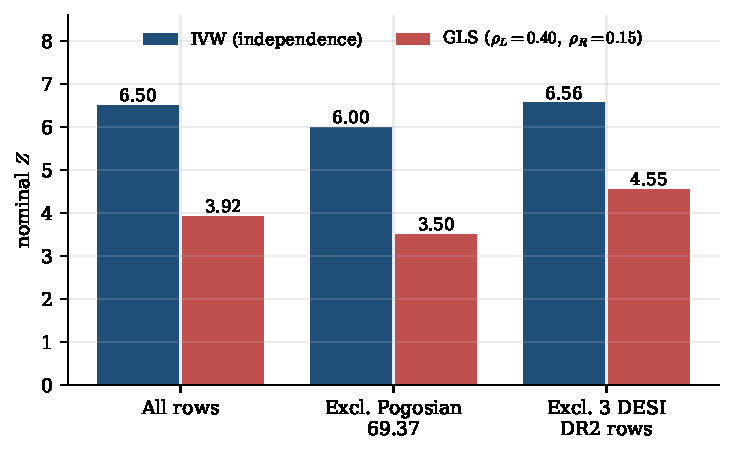
\includegraphics[width=.62\linewidth]{figures/fig_scenarios.pdf}
\caption{Nominal $Z$ across the six scenarios of \cref{tab:scen}; conditional on the stated estimator and covariance assumptions.}\label{fig:scen}
\end{figure}
\begin{figure}[t]\centering
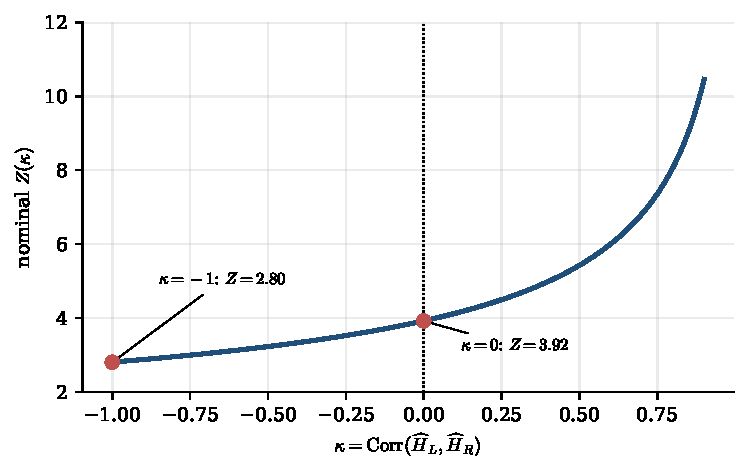
\includegraphics[width=.62\linewidth]{figures/fig_kappa.pdf}
\caption{$Z(\kappa)$ for the GLS contrast of \cref{tab:base} (\cref{prop:kappa}). Positive cross-group correlation raises $Z$.}\label{fig:kappa}
\end{figure}
\begin{figure}[t]\centering
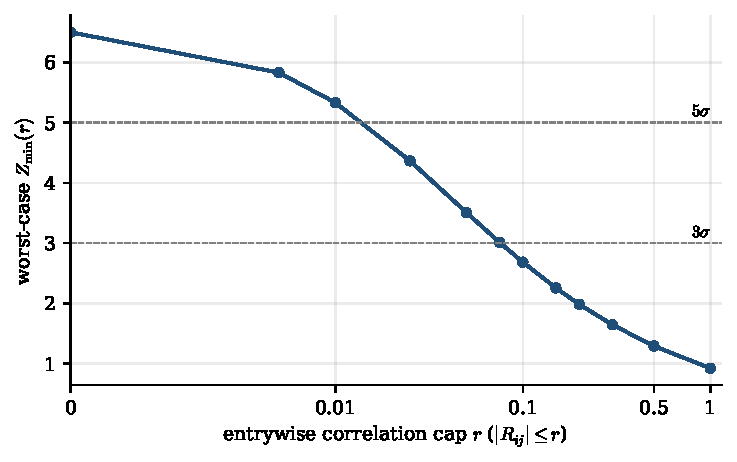
\includegraphics[width=.62\linewidth]{figures/fig_cap.pdf}
\caption{Worst-case $Z_{\min}(r)$ under an entrywise correlation cap (\cref{prop:cap}), for fixed inverse-variance weights.}\label{fig:cap}
\end{figure}
\begin{figure}[t]\centering
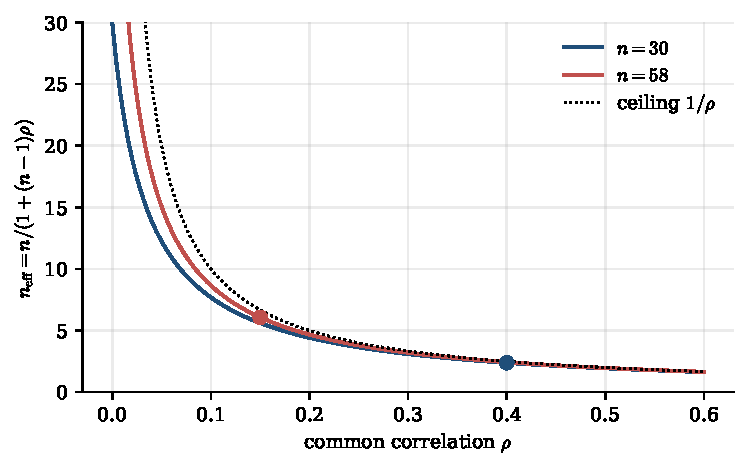
\includegraphics[width=.62\linewidth]{figures/fig_deff.pdf}
\caption{Effective number of independent estimates for equal errors (\cref{prop:deff}); dots mark the two assumed $(n,\rho)$ pairs.}\label{fig:deff}
\end{figure}

\section{Application to a reconstruction of the 88-row table}\label{sec:app}
\paragraph{Reconstruction.} The pinned upstream repository could not be retrieved in the environment used to prepare this paper, so the 88 rows were rebuilt from Appendix~A of the source paper (arXiv:2601.00650v2, Tables~X and~XI), with asymmetric errors reduced by the paper's own RMS rule. Of the 88 rows, 55 are exact as printed, 27 are RMS-symmetrised from two printed errors, and 6 carry one error component that was unreadable in the extracted text and is estimated (\texttt{status=approx} in \texttt{data/h0\_compilation\_reconstructed.csv}); the Dominguez et al.\ and Gonzalez et al.\ entries were additionally checked against their published abstracts. The reconstruction is validated against the packaged results (\cref{tab:valid}): the ladder group is reproduced to machine precision, and the comparison group to $0.0034\unit$ in the IVW mean. It is nevertheless provisional; the authoritative table is the one fetched from the pinned commit (\texttt{make data}), and every number in this section should be regenerated from it before submission.
\begin{table}[t]\centering\small
\caption{Reconstruction versus packaged results (units $\kmsMpc$).}\label{tab:valid}
\begin{tabular}{@{}lccc@{}}\toprule
Quantity & Reconstructed & Packaged & $|\Delta|$\\\midrule
IVW ladder mean & 72.732465 & 72.732465 & 0\\
GLS ladder mean $\pm$ SE & $72.302030\pm0.571293$ & $72.302030\pm0.571293$ & 0\\
IVW comparison mean & 69.375633 & 69.372226 & 0.0034\\
IVW comparison SE & 0.345137 & 0.344887 & 0.0003\\
GLS comparison mean & 69.521464 & 69.520526 & 0.0009\\
GLS comparison SE & 0.420127 & 0.420384 & 0.0003\\
Negative weights (ladder / comparison) & 16 / 38 & 16 / 38 & 0\\\bottomrule
\end{tabular}\end{table}

\paragraph{Negative weights are explained by \cref{cor:neg}.} For $(\rho_L,\rho_R)=(0.40,0.15)$ the thresholds are $s^\ast_L=2.536$ and $s^\ast_R=4.218\unit$: exactly the 16 ladder rows with $s_i>2.536$ and the 38 comparison rows with $s_i>4.218$ receive negative weight.

\paragraph{Feasible cross-group correlation.} Across the exact PSD interval $|\rho_{LR}|\le0.2630$ the correlation between the two pooled means is $|\kappa|\le0.098$, and the GLS contrast varies only between $Z=3.749$ ($\rho_{LR}=-0.263$) and $Z=4.119$ ($+0.263$), through $Z=3.921$ at $0$. The envelope $2.80\le Z\le18.4$ of \cref{prop:kappa} is therefore far wider than anything attainable by a constant cross-group correlation consistent with the assumed within-group structure.

\paragraph{Cap bound.} The sharp bound of \cref{prop:cap}, evaluated on the reconstruction, gives $Z_{\min}=6.49,\,5.32,\,4.36,\,3.51,\,2.68,\,1.98,\,1.29,\,0.92$ for $r=0,\,0.01,\,0.025,\,0.05,\,0.10,\,0.20,\,0.50,\,1$, matching the packaged values of Section~\ref{sec:cap} to better than $0.01$ and equalling them at $r=1$: an independent confirmation of both the formula and the legacy script.

\paragraph{Random correlation structures.} \Cref{tab:lkj} reports $Z=|\widehat\Delta|/\sqrt{q^{\!\top}Rq}$ for the fixed inverse-variance estimator when $R$ is drawn from LKJ($\eta$) over all 88 rows (``joint'') or independently within each group (``block''), 40\,000 draws each. Consistently with \cref{prop:lkj}, the distribution is narrow and centred on the independence value $6.5$.
\begin{table}[t]\centering\small
\caption{Prior-predictive $Z$ under LKJ($\eta$) correlation matrices (reconstructed table; fixed IVW weights; seed 20261026).}\label{tab:lkj}
\begin{tabular}{@{}lcccc@{}}\toprule
Structure & $\eta$ & median $Z$ & 95\% interval & $P(Z>5)$\\\midrule
joint & 1 & 6.52 & [5.68, 7.57] & $>0.9999$\\
joint & 2 & 6.51 & [5.69, 7.57] & $>0.9999$\\
joint & 5 & 6.51 & [5.71, 7.52] & $>0.9999$\\
joint & 20 & 6.51 & [5.80, 7.38] & $>0.9999$\\
block & 2 & 6.52 & [5.65, 7.62] & $>0.9999$\\\bottomrule
\end{tabular}\end{table}
The contrast between \cref{tab:lkj} and the equicorrelated value $3.92$ is the central quantitative message: \emph{the significance is not lost to dependence in general; it is lost to a specific assumption, namely positive correlation of equal sign across every pair in each group.} Whether such coherent shared systematics exist at the assumed strength is an empirical question that the covariance products of the primary analyses, not a prior over correlation matrices, must answer.

\section{Provenance of the \texorpdfstring{$69.37\pm0.65$}{69.37 +/- 0.65} entry and DESI DR2 overlap}\label{sec:prov}
The repository row labels this estimate 2024 and cites arXiv:2405.20306~\cite{Pogosian2024}, whose abstract reports $69.48\pm0.94\unit$ for DESI Year-1. A public presentation dated July 2025~\cite{PogosianPASCOS2025} reports $69.37\pm0.65\unit$ from DESI DR2 BAO, the CMB acoustic scale and a Gaussian Planck prior on $\omega_m$, with the sound horizon free. The source paper describes the entry as a 2025 seminar/private-communication result with publication forthcoming. The matching number thus has a plausible DR2-era description, but the repository metadata does not link the row to it. \emph{This is a traceability mismatch, not evidence of a numerical error or of misconduct}, and it is recorded as unresolved pending the authors' response.

Three comparison rows use DESI DR2 inputs: $69.37\pm0.65$, $70.03\pm0.97$~\cite{GarciaEscudero2025} and $71.59\pm0.94$~\cite{Du2025}. Their shares of the comparison group's diagonal inverse-variance weight are $28.15\%$, $12.64\%$ and $13.46\%$, totalling $54.26\%$. That figure is a property of naive diagonal weighting. Shared DESI DR2 BAO data do not by themselves fix a pairwise covariance, which also depends on the additional likelihoods and nuisance parameters; neither independence nor perfect correlation is justified (see also \cite{H0DN2026} for a covariance-weighted treatment of local distance indicators and \cite{Hedges2010} for robust variance estimation with dependent estimates).

\section{Software and reproducibility}\label{sec:software}
All results of \cref{sec:theory} are implemented in a header-only C++17 library with a command-line tool and mirrored in a NumPy package. Unit tests check: closed form versus dense Cholesky GLS; the negative-weight threshold; the design effect; the PSD limit (feasible just inside, infeasible just outside); the cap bound (attained, and never exceeded by random feasible matrices); and agreement of the two implementations to relative $10^{-9}$.

A prior-predictive tool draws LKJ($\eta$) correlation matrices~\cite{LKJ2009} by the C-vine construction (the draw is validated against the known marginal variance $1/(2\eta-1+d)$) and returns the distribution of $Z$ for fixed estimator weights; it is bit-reproducible for any thread count. It is intended for sensitivity exploration, not as a physical model of the dependence. Timing on a synthetic fixture with $d=88$ and $\eta=2$ on one core was about $0.6$~ms per draw in C++ versus $89$~ms in Python (about $150\times$). Its application to the reconstructed table is reported in \cref{sec:app}; the same command reproduces it on the authoritative table after \texttt{make data}.

\section{Limitations}
(i) The analysis is summary-level, not a joint-likelihood refit of the primary BAO, CMB, supernova, lensing or distance-ladder data. (ii) The joint covariance of the 88 estimates is not available; $\rho_L,\rho_R$ are the source paper's illustrative values. (iii) Cross-group covariance is set to zero except where explicitly varied. (iv) Asymmetric errors are symmetrised as upstream, discarding non-Gaussian information. (v) Exclusion scenarios keep $\rho_R$ fixed. (vi) The provenance audit is targeted (one entry and three DESI DR2-related rows), not a row-by-row audit of all 88. (vii) Section~\ref{sec:app} uses a provisional reconstruction of the table (six rows with an estimated error component), not the pinned upstream file. (viii) Gaussianity is assumed throughout, and the nominal $Z$ is not a calibrated $p$-value under covariance uncertainty.

\section{Conclusions}
The reproduced inverse-variance contrast of $6.50\sigma$ falls to $3.92\sigma$ under the source paper's assumed within-group correlations, but that number is conditional on the estimator, on $(\rho_L,\rho_R)$, and on setting the cross-group covariance to zero. The paper's mathematical contribution is to make those dependencies explicit and checkable: exact weights and their signs, the information ceiling $1/\rho$, the admissible range $|\rho_{LR}|\le0.263$, the monotone dependence on $\kappa$, and a sharp worst-case bound for any stated correlation cap. On the reconstructed table, generic random dependence leaves the independence significance nearly intact ($Z\in[5.7,7.6]$), so the reduction to $3.9$ rests on a specific sign-coherent correlation structure whose strength is assumed, not measured. A decisive treatment requires a row-level provenance table for all 88 entries, an overlap graph at likelihood level, and either joint covariance products or pre-specified bounds on defensible covariance structures. Until then, the tension is neither dismissed nor given a covariance-free significance.

\section*{Declarations}
\noindent\textbf{Data and code availability.} Source data: the pinned repository snapshot of Section~\ref{sec:data}; the reconstructed table used in Section~\ref{sec:app} is in the companion repository with per-row status flags. Code, tests, packaged tables and figure scripts: companion repository \texttt{h0-covariance-audit} (release 1.0.0; archive DOI to be added at deposit).\\
\textbf{Competing interests.} None declared. \textbf{Funding.} No external funding.\\
\textbf{Use of AI tools.} [Author to complete according to the target journal's policy.]\\
\textbf{Scope and submission status.} Technical note; to be submitted only after the checks listed in \texttt{docs/PRE\_SUBMISSION\_CHECKLIST.md} are complete.

\bibliographystyle{unsrtnat}
\bibliography{references}
\end{document}
